\section{Overview}
This supplement provides the score-contrast derivation, inference settings,
design controls, reference-data protocol, and complete numerical records.
It accompanies the initial 40-reference study and expanded development
comparisons in the main paper.
The frozen multi-seed test is being generated, and its final results will
use the same pairing and metric definitions.

New references have identifiers prefixed by \texttt{kr\_dev} and
\texttt{kr\_test}. The initial 40-reference, single-prompt/seed study has a separate section
with complete per-reference measurements.
That archive contains 160 stored measurements. The original output images
and complete run/evaluator records are not all recovered, so the archived
table and new experiments have separate provenance.

\section{Derivation of the latent objective}
\subsection{Conditioning and score conversion}
Let $r$ be the reference and $c$ the full target instruction. At the same
state $z_\sigma$, define $v_r=v_\theta(z_\sigma,\sigma,c,r)$ and
$v_b=v_\theta(z_\sigma,\sigma,c,\varnothing)$. Removing the reference
does not remove the text. Target geometry, latent, and noise level are
shared. Both predictions use frozen weights and are detached during latent
optimization.

For $z_\sigma=(1-\sigma)x_0+\sigma\epsilon$, with Gaussian $\epsilon$,
the conditional-mean flow velocity obeys
\begin{equation}
v(z_\sigma,\sigma)=\mathbb E[\epsilon-x_0\mid z_\sigma].
\end{equation}
The conditional Gaussian-noise score identity is
$s(z_\sigma,\sigma)=-\mathbb E[\epsilon\mid z_\sigma]/\sigma$.
Taking the conditional mean of
$z_\sigma+(1-\sigma)(\epsilon-x_0)=\epsilon$ therefore gives
\begin{equation}
s_\theta=-\frac{z_\sigma+(1-\sigma)v_\theta}{\sigma}.
\end{equation}
The learned velocity approximates this conditional-mean field. Subtracting the two conditions cancels the state term:
\begin{equation}
\Delta s=s_r-s_b=-\frac{1-\sigma}{\sigma}(v_r-v_b).
\end{equation}
For a positive noise level below one, the velocity-to-score contrast factor
is negative. Optimization is omitted at the terminal zero-noise state,
and the numerical implementation clamps small denominators.

\subsection{Detach, reduction and update magnitude}
For each sample with $N$ latent elements, let $g=a\Delta s$, $a>0$, and
\begin{equation}
d=\frac{g}{\max(\sqrt{N^{-1}\sum_jg_j^2},\varepsilon_g)}.
\end{equation}
The primary branch uses a detached velocity to define
\begin{align}
\hat x_0(z)&=z-\sigma\sg(v_b),\\
y&=\sg(\hat x_0(z)+\eta d),\\
L_p&=\frac{1}{2N}\sum_j(\hat x_{0,j}(z)-y_j)^2.
\end{align}
Both $d$ and $y$ are treated as constants during differentiation. Hence
\begin{equation}
\frac{\partial\hat x_0}{\partial z}=I,
\qquad\nabla_zL_p=-\frac{\eta}{N}d.
\end{equation}
The identity Jacobian follows from detaching $v_b$ in this branch. Without
that detach, an additional velocity Jacobian would enter. The factor $1/N$
follows from mean reduction and must not be dropped when interpreting SGD.

Plain SGD with learning rate $\ell$ and no other losses produces
$\Delta z=\ell\eta d/N$. Adam or AdamW instead rescales gradients using
moment estimates and numerical stabilization. Thus $\eta$ fixes a target
offset, not an optimizer displacement. Positive multipliers cancel in RMS
normalization away from the numerical floor. We record actual update RMS
to characterize displacement under the chosen optimizer and precision.

For the evaluated AdamW setting, weight decay is zero. Let
$h_k=\nabla_zL_p$ at inner iteration $k$. Starting from $m_0=u_0=0$ at each
outer intervention, the elementwise update is
\begin{align}
m_k&=\beta_1m_{k-1}+(1-\beta_1)h_k,\\
u_k&=\beta_2u_{k-1}+(1-\beta_2)h_k^2,\\
\hat m_k&=m_k/(1-\beta_1^k),\qquad
\hat u_k=u_k/(1-\beta_2^k),\\
z_{k+1}&=z_k-\ell\frac{\hat m_k}{\sqrt{\hat u_k}+\epsilon_{\rm opt}}.
\end{align}
The implementation uses the optimizer defaults
$\beta_1=.9$, $\beta_2=.999$, and $\epsilon_{\rm opt}=10^{-8}$.
These moments persist within an intervention and are reset at the next
outer intervention. The gradient scale and target offset therefore do not
specify a fixed latent displacement.

\section{Execution order and controls}
\subsection{Reverse-first alternation}
At each actual solver interval, the frozen reverse step first reaches the
next noise level. An eligible positive reached node is then assigned its
inner latent updates. The teacher predictions are recomputed after each
latent change at that same noise level. A new latent optimizer is created
for each outer intervention. Its state persists within that intervention.
The final reverse interval has no subsequent inner update.

The evaluated operator uses only the pseudo-target objective. Distribution
and content-loss weights are zero, and SLT, warm-start AdaIN, and final
AdaIN are disabled. Earlier archived settings have separate configuration
provenance.

\subsection{Separate text guidance from reference guidance}
Sampler text CFG forms
\begin{equation}
v^\beta=v_{\rm uncond}+\beta(v_{\rm cond}-v_{\rm uncond}).
\end{equation}
Direct reference CFG forms
\begin{equation}
v_{\rm refCFG}=v_b^\beta+\gamma(v_r^\beta-v_b^\beta).
\end{equation}
The native reference control at $\gamma=1$ evaluates only the reference
branch, and its cost reflects those evaluations. The current protocol records sampler text CFG $\beta=4$, a
style-contrast CFG parameter of 4, and embedded guidance 0 as separate
settings. The code forms the positive score multiplier as
$a=\lambda_{\rm CA}(4-1)=3$ with $\lambda_{\rm CA}=1$ before RMS
normalization.

\subsection{Development controls and comparison settings}
The same-backbone controls use a frozen Klein-9B-base pipeline at
$512\times512$, with layer-wise CPU offload and a requested 12-GiB
model-memory budget. The common-node variants use one inner update at
$\mathcal G=\{.8,.6,.4,.2\}$, AdamW at learning rate .01, zero weight
decay, and target offset .05. Inserting these nodes yields 29 actual
intervals for a nominal 25-step solver and 12 for a nominal eight-step
solver. The RMS-SGD control normalizes latent-gradient RMS before an SGD
step at rate .01. Measured displacement is retained for each optimizer.

Dense variants use the original positive solver nodes. The 25-step
variants vary inner count and learning rate at target offset .05. The
eight-step/K5 setting uses target offset .12. Dense25/K5 requires 290 DiT
forwards and 120 latent backward calls, compared with 146/48 for the
retained 25/K2 and 86/35 for 8/K5. All use text CFG 4. Direct-reference
controls vary reference scale and reverse-step budget, with actual model
calls recorded for every output.

AD uses SD1.5, 50 steps, two inner updates, learning rate .015, text CFG
7.5, AdaIN, and bf16. USO uses the style-only FLUX.1-dev interface with
pretrained rank-128 LoRA/projector and SigLIP, 25 steps, guidance 4, FP8
weight storage, and bf16 computation. Its content-image input is empty.
The backbone, adapter, precision, and offload configuration accompany each
method's results.

StyleShot uses the official SD1.5 pipeline, a pretrained style encoder and
image adapter, style scale 1, text CFG 7.5, and float32 inference. Its PNDM
scheduler has 51 actual evaluation nodes at a nominal 50-step setting.
The negative prompt is ``monochrome, lowres, bad anatomy, worst quality, low
quality''. The random seed initializes both image sampling and the
style-encoder patch permutation. We use the same reference-plus-text inputs
and seed-64 grid as the other methods.

InstantStyle uses the official SDXL style-only block
\texttt{up\_blocks.0.attentions.1}, with adapter scale 1, text CFG 5,
30 Euler steps, and float16 inference. Its target text appends
``masterpiece, best quality, high quality''. The official negative prompt
is ``text, watermark, lowres, low quality, worst quality, deformed, glitch,
low contrast, noisy, saturation, blurry''. Image projection and attention
adapter parameters pass strict state-dictionary loading. Existing SDXL
weights are reused through a local directory view, with no weight changes.

\subsection{Complete development comparisons}
The search contains 400 outputs from 25 configurations on four development
references, two prompts, and two seeds (Table~\ref{tab:searchcomplete}).
The initial coverage grid contains 240 outputs from five candidates on
eight development references, six prompts, and seed 64. Adding StyleShot
and InstantStyle on the identical 48 cells each gives the 336-output comparison
(Table~\ref{tab:coveragecomplete}). Every configuration covers the same
cells within its grid. Exact common cells are reused between stages, so
the search and coverage counts overlap. All outputs have the three
reported metric readouts.

Single- and two-GPU placements share the same model precision and method
settings. The two-GPU implementation was checked against a single-GPU
reference on a full generation case, with pixel-identical output. Placement
and timing are recorded separately.

\begin{table*}[t]
\centering\small
\caption{Complete development search: 25 configurations, each with four
references, two prompts, and two seeds (16 outputs). ``Four nodes'' denotes
one update at each common intervention node. ``+nodes'' denotes node
insertion into the nominal solver. Labels map to experiment identifiers in
the source records.}
\label{tab:searchcomplete}
\begin{tabular}{lrrr}
\toprule
Configuration & CSD $\uparrow$ & CLIP-T $\uparrow$ & Layout \\
\midrule
AD (SD1.5) & 0.6789 & 0.2894 & 0.3963 \\
USO (FLUX.1, FP8) & 0.3378 & 0.3244 & 0.3587 \\
TSD25, four nodes & 0.0386 & 0.3190 & 0.3398 \\
TSD25, K1 & 0.3726 & 0.3109 & 0.3665 \\
TSD, 25/K2 & 0.5555 & 0.3110 & 0.4350 \\
TSD25, K5, $\ell=.005$ & 0.6288 & 0.2986 & 0.4941 \\
TSD8, four nodes & 0.0315 & 0.3168 & 0.3465 \\
TSD25, K5 & 0.7302 & 0.2796 & 0.5955 \\
TSD, 8/K5 & 0.3891 & 0.3110 & 0.3754 \\
TSD25, four nodes, $\ell=.005$ & 0.0341 & 0.3198 & 0.3394 \\
TSD25, four nodes, $\ell=.02$ & 0.0468 & 0.3191 & 0.3404 \\
Native global & 0.0633 & 0.3100 & 0.3411 \\
Native semantic & 0.0809 & 0.3070 & 0.3516 \\
Ref. CFG144, $\gamma=1$ & 0.1401 & 0.3133 & 0.3524 \\
Ref. CFG72, $\gamma=3$ & 0.2545 & 0.3185 & 0.3810 \\
Reference CFG, 72/$\gamma=5$ & 0.2631 & 0.3114 & 0.4137 \\
Ref. CFG12+nodes, $\gamma=.5$ & 0.0635 & 0.3145 & 0.3386 \\
Ref. CFG12+nodes, $\gamma=1.5$ & 0.1865 & 0.3163 & 0.3616 \\
Ref. CFG25+nodes, $\gamma=.5$ & 0.0682 & 0.3163 & 0.3421 \\
Ref. CFG25+nodes, $\gamma=1.5$ & 0.1862 & 0.3159 & 0.3587 \\
Ref. CFG25+nodes, $\gamma=2$ & 0.2227 & 0.3170 & 0.3650 \\
Ref. CFG25+nodes, $\gamma=3$ & 0.2517 & 0.3185 & 0.3799 \\
Ref. CFG25+nodes, $\gamma=5$ & 0.2470 & 0.3147 & 0.4092 \\
Ref. CFG25+nodes, $\gamma=1$ & 0.1247 & 0.3150 & 0.3522 \\
RMS-SGD, four nodes & 0.0411 & 0.3186 & 0.3397 \\
\bottomrule
\end{tabular}

\end{table*}

\begin{table}[t]
\centering\small
\caption{Expanded development comparison: seven settings on eight
references, six prompts, and seed 64 (48 outputs per row).}
\label{tab:coveragecomplete}
\resizebox{\columnwidth}{!}{\begin{tabular}{lrrr}
\toprule
Method & CSD $\uparrow$ & CLIP-T $\uparrow$ & Layout \\
\midrule
Reference CFG, 72/$\gamma=5$ & 0.3190 & 0.3005 & 0.3118 \\
AD (SD1.5) & 0.7069 & 0.2692 & 0.3224 \\
USO (FLUX.1, FP8) & 0.4117 & 0.3178 & 0.2953 \\
StyleShot (SD1.5) & 0.5042 & 0.2840 & 0.2703 \\
InstantStyle (SDXL) & 0.4947 & 0.2616 & 0.2900 \\
TSD, 8/K5 & 0.4291 & 0.3078 & 0.3101 \\
TSD, 25/K2 & 0.5751 & 0.2982 & 0.3503 \\
\bottomrule
\end{tabular}
}
\end{table}

\subsection{Why use a moderate inner-update count?}
We vary the inner-update count while keeping the 25-step solver, learning
rate .01, target offset .05, backbone, and input cells fixed. K1, K2, and
K5 use the same four references, two prompts, and two seeds (16 outputs
per setting). K1 gives lower style similarity. Increasing the count to K5
strengthens the reference style but reduces target-text alignment. K2
retains stronger style than K1 with similar CLIP-T and uses fewer forward
calls than K5 (Table~\ref{tab:densitychoice}). This comparison motivates the
25/K2 working point used in the formal protocol.

\begin{table}[t]
\centering\small
\caption{Inner-update count at fixed 25-step settings. Means over the same
16 development cells. Forward calls count DiT evaluations per output.}
\label{tab:densitychoice}
\begin{tabular}{lrrr}
\toprule
Updates & CSD $\uparrow$ & CLIP-T $\uparrow$ & Forwards \\
\midrule
K1 & .3726 & .3109 & 98 \\
K2 & .5555 & .3110 & 146 \\
K5 & .7302 & .2796 & 290 \\
\bottomrule
\end{tabular}
\end{table}

Reducing the K5 learning rate to .005 gives CSD .6288 and CLIP-T .2986,
compared with .5555/.3110 for K2 at .01. This control shows that reducing
update count and reducing learning rate yield different operating points.
The full search table preserves both alternatives. The recorded outputs support paired qualitative inspection of medium
appearance and subject structure under these settings.

\begin{figure}[t]
\centering
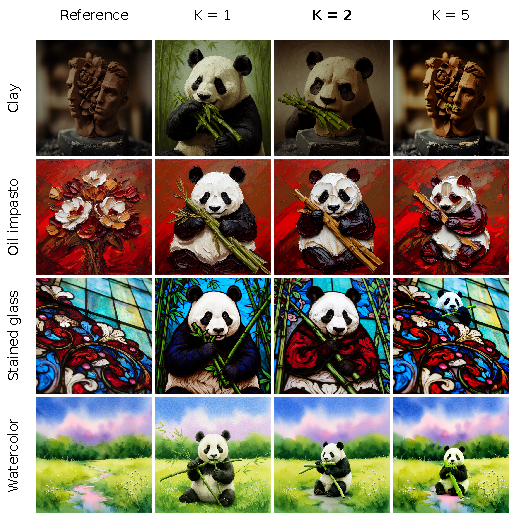
\includegraphics[width=\columnwidth]{inner_update_ablation.pdf}
\caption{Effect of inner-update count at fixed 25-step sampling,
learning rate .01, and target offset .05. Rows cover all four references
in the configuration study, using the panda prompt and seed 64. K1, K2,
and K5 share the same initial seed and reference. Increasing the update
count strengthens the reference appearance, while K2 retains a clearer
panda than K5 in the clay example. Table~\ref{tab:densitychoice} reports
means over both prompts and both seeds.}
\label{fig:innercount}
\end{figure}

Figure~\ref{fig:innercount} shows the visual role of update count on the
same references. The comparison varies only $K$, keeping the solver and
optimizer settings fixed. It explains the choice of a moderate update
budget alongside the complete-grid measurements.

\subsection{Frozen held-out evaluation}
After the complete development checks, protocol \texttt{cvpr\_test\_v1}
freezes 40 disjoint test references, six literal prompts, seeds 64/65/66,
and five settings before generating test outputs (720 per setting, 3,600
total). TSD8/K5 uses eight intervals, five updates, target offset .12, and
learning rate .01. TSD25/K2 uses 25 intervals, two updates, target offset
.05, and learning rate .01. Both use text CFG 4 and disable auxiliary
distribution/content losses, SLT, and AdaIN. The direct control uses 72
intervals and reference scale five. AD and USO retain their documented
development settings. Sources, input hashes, model-file identities, and
the full cell matrix are frozen. No test result is used to tune parameters.
The test is running, not complete, in this working supplement.

\section{Reference data and metric definitions}
\subsection{New collection and split}
The new Krea collection contains 48 public-feed synthetic references,
visually selected for medium clarity, quality, and content diversity before
method outputs were examined. Each of eight medium categories contributes
one development and five test references (Table~\ref{tab:categories}).
Studio/tool photographs, dominant gallery frames, multi-panel collages,
and ambiguous media were excluded during reference curation, not according
to method success. The category labels describe the visual appearance of these synthetic
references.

\begin{table}[t]
\centering\small
\caption{New synthetic-reference split, distinct from the archived 40 IDs.}
\label{tab:categories}
\begin{tabular}{lcc}
\toprule
Medium category & Development & Test \\
\midrule
clay & 1 & 5 \\
colored\_pencil & 1 & 5 \\
mosaic & 1 & 5 \\
oil\_impasto & 1 & 5 \\
stained\_glass & 1 & 5 \\
paper\_cut & 1 & 5 \\
watercolor & 1 & 5 \\
woodcut & 1 & 5 \\
\midrule
Total & 8 & 40 \\
\bottomrule
\end{tabular}

\end{table}

All methods receive the same 512-by-512 RGB reference, obtained by
aspect-preserving Lanczos resizing and center cropping of the public
1024-pixel image version. The manifest records source UUIDs and URLs,
source/derived hashes, split, and transform. The numeric and protocol package contains source metadata. It does not
redistribute the raw reference images.

\subsection{Readouts and their limitations}
CSD is cosine similarity between style descriptors of an output and its
reference \citep{somepalli2024csd}. CLIP-T is image--text cosine similarity
to the target content request without the style-instruction wrapper
\citep{radford2021clip}. Reference-layout similarity is Pearson correlation
between off-diagonal patch self-similarity vectors from DINO features
\citep{oquab2024dinov2}. Higher layout similarity is task-dependent and may
reflect shared semantics as well as geometry. None of these scores alone
establishes successful transfer or image quality.

For new evaluation, the implemented protocol specifies the official CSD
ViT-L checkpoint, OpenAI CLIP ViT-B/32, and timm DINOv2 ViT-B/14.
CSD inputs use bilinear 224-pixel resizing and CLIP normalization. CLIP-T
uses the model's standard preprocessing. DINO inputs use bilinear
518-pixel resizing and ImageNet normalization. The evaluator is designed to
record checkpoint hashes and require strict state-dict loading. All three
metrics executed with validated weights. The earlier archive retains its
own evaluator-provenance qualification.

\section{Complete archived per-reference measurements}
Tables~\ref{tab:allcsd}--\ref{tab:alllayout} retain every reference ID and
all four methods for the three reported readouts. TSD-S/TSD-G map to
archived identifiers \texttt{q25s}/\texttt{pg\_n8\_s12\_r}. Native-S/Native-G
map to \texttt{kleinsys\_sem}/\texttt{kleinsys\_gst}. Values are rounded
only for display. The numeric export retains the stored precision.

\begin{table*}[t]
\centering\small
\caption{All archived CSD measurements, one prompt and seed 65.}
\label{tab:allcsd}\begin{tabular}{ccccc@{\hspace{14pt}}ccccc}
\toprule
Style & TSD-S & Native-S & TSD-G & Native-G & Style & TSD-S & Native-S & TSD-G & Native-G \\
\midrule
00 & 0.698 & 0.507 & 0.700 & 0.519 & 20 & 0.657 & 0.344 & 0.546 & 0.312 \\
01 & 0.759 & 0.482 & 0.731 & 0.433 & 21 & 0.703 & 0.110 & 0.547 & 0.101 \\
02 & 0.668 & -0.020 & 0.532 & 0.010 & 22 & 0.720 & 0.484 & 0.756 & 0.478 \\
03 & 0.819 & 0.283 & 0.699 & 0.239 & 23 & 0.612 & 0.268 & 0.603 & 0.141 \\
04 & 0.813 & 0.077 & 0.634 & 0.003 & 24 & 0.758 & 0.083 & 0.747 & 0.085 \\
05 & 0.770 & 0.462 & 0.596 & 0.463 & 25 & 0.603 & 0.423 & 0.529 & 0.434 \\
06 & 0.659 & 0.043 & 0.529 & 0.079 & 26 & 0.622 & 0.356 & 0.554 & 0.338 \\
07 & 0.527 & 0.211 & 0.475 & 0.246 & 27 & 0.757 & 0.259 & 0.593 & 0.183 \\
08 & 0.702 & 0.007 & 0.591 & 0.028 & 28 & 0.726 & 0.385 & 0.696 & 0.291 \\
09 & 0.795 & 0.415 & 0.692 & 0.144 & 29 & 0.668 & 0.328 & 0.559 & 0.203 \\
10 & 0.683 & 0.166 & 0.437 & 0.182 & 30 & 0.590 & 0.216 & 0.494 & 0.235 \\
11 & 0.784 & 0.400 & 0.696 & 0.403 & 31 & 0.700 & 0.102 & 0.611 & 0.109 \\
12 & 0.838 & 0.518 & 0.767 & 0.279 & 32 & 0.886 & 0.461 & 0.788 & 0.528 \\
13 & 0.635 & 0.134 & 0.620 & 0.172 & 33 & 0.721 & 0.284 & 0.589 & 0.280 \\
14 & 0.804 & 0.327 & 0.672 & 0.303 & 34 & 0.729 & 0.426 & 0.721 & 0.448 \\
15 & 0.802 & 0.148 & 0.711 & 0.101 & 35 & 0.712 & 0.278 & 0.605 & 0.278 \\
16 & 0.774 & -0.006 & 0.473 & 0.023 & 36 & 0.781 & 0.573 & 0.657 & 0.601 \\
17 & 0.735 & 0.159 & 0.683 & 0.144 & 37 & 0.655 & 0.321 & 0.596 & 0.314 \\
18 & 0.764 & -0.012 & 0.505 & 0.048 & 38 & 0.839 & 0.139 & 0.718 & 0.259 \\
19 & 0.671 & 0.317 & 0.469 & 0.289 & 39 & 0.629 & 0.227 & 0.467 & 0.175 \\
\bottomrule
\end{tabular}

\end{table*}
\begin{table*}[t]
\centering\small
\caption{All archived CLIP-T measurements, one prompt and seed 65.}
\label{tab:allclip}\begin{tabular}{ccccc@{\hspace{14pt}}ccccc}
\toprule
Style & TSD-S & Native-S & TSD-G & Native-G & Style & TSD-S & Native-S & TSD-G & Native-G \\
\midrule
00 & 0.309 & 0.319 & 0.308 & 0.313 & 20 & 0.308 & 0.317 & 0.317 & 0.331 \\
01 & 0.314 & 0.300 & 0.289 & 0.323 & 21 & 0.302 & 0.317 & 0.311 & 0.312 \\
02 & 0.299 & 0.305 & 0.293 & 0.305 & 22 & 0.288 & 0.332 & 0.310 & 0.322 \\
03 & 0.326 & 0.313 & 0.271 & 0.314 & 23 & 0.277 & 0.346 & 0.290 & 0.314 \\
04 & 0.253 & 0.324 & 0.314 & 0.305 & 24 & 0.306 & 0.322 & 0.314 & 0.316 \\
05 & 0.283 & 0.331 & 0.284 & 0.343 & 25 & 0.325 & 0.328 & 0.322 & 0.331 \\
06 & 0.345 & 0.308 & 0.336 & 0.302 & 26 & 0.320 & 0.337 & 0.343 & 0.344 \\
07 & 0.324 & 0.311 & 0.308 & 0.316 & 27 & 0.261 & 0.310 & 0.293 & 0.312 \\
08 & 0.312 & 0.329 & 0.306 & 0.317 & 28 & 0.345 & 0.338 & 0.317 & 0.308 \\
09 & 0.230 & 0.296 & 0.224 & 0.312 & 29 & 0.306 & 0.331 & 0.347 & 0.318 \\
10 & 0.327 & 0.311 & 0.312 & 0.309 & 30 & 0.321 & 0.317 & 0.328 & 0.315 \\
11 & 0.217 & 0.318 & 0.299 & 0.305 & 31 & 0.320 & 0.322 & 0.301 & 0.323 \\
12 & 0.300 & 0.326 & 0.296 & 0.325 & 32 & 0.217 & 0.309 & 0.209 & 0.309 \\
13 & 0.324 & 0.304 & 0.316 & 0.309 & 33 & 0.301 & 0.319 & 0.300 & 0.299 \\
14 & 0.277 & 0.330 & 0.282 & 0.305 & 34 & 0.281 & 0.304 & 0.284 & 0.296 \\
15 & 0.269 & 0.314 & 0.296 & 0.306 & 35 & 0.272 & 0.289 & 0.293 & 0.308 \\
16 & 0.302 & 0.331 & 0.332 & 0.309 & 36 & 0.274 & 0.326 & 0.323 & 0.334 \\
17 & 0.309 & 0.314 & 0.308 & 0.304 & 37 & 0.310 & 0.313 & 0.331 & 0.331 \\
18 & 0.283 & 0.327 & 0.301 & 0.326 & 38 & 0.269 & 0.328 & 0.335 & 0.317 \\
19 & 0.308 & 0.331 & 0.304 & 0.313 & 39 & 0.303 & 0.306 & 0.302 & 0.314 \\
\bottomrule
\end{tabular}

\end{table*}
\begin{table*}[t]
\centering\small
\caption{All archived reference-layout similarity measurements. Desirability
depends on the requested task. One prompt and seed 65.}
\label{tab:alllayout}\begin{tabular}{ccccc@{\hspace{14pt}}ccccc}
\toprule
Style & TSD-S & Native-S & TSD-G & Native-G & Style & TSD-S & Native-S & TSD-G & Native-G \\
\midrule
00 & 0.448 & 0.385 & 0.341 & 0.376 & 20 & 0.345 & 0.355 & 0.370 & 0.322 \\
01 & 0.735 & 0.346 & 0.672 & 0.419 & 21 & 0.449 & 0.351 & 0.365 & 0.324 \\
02 & 0.359 & 0.303 & 0.327 & 0.281 & 22 & 0.533 & 0.260 & 0.318 & 0.287 \\
03 & 0.697 & 0.291 & 0.571 & 0.220 & 23 & 0.373 & 0.265 & 0.288 & 0.260 \\
04 & 0.590 & 0.333 & 0.430 & 0.364 & 24 & 0.388 & 0.246 & 0.310 & 0.244 \\
05 & 0.803 & 0.327 & 0.542 & 0.393 & 25 & 0.474 & 0.374 & 0.409 & 0.348 \\
06 & 0.620 & 0.372 & 0.512 & 0.363 & 26 & 0.526 & 0.342 & 0.392 & 0.338 \\
07 & 0.482 & 0.380 & 0.433 & 0.368 & 27 & 0.546 & 0.330 & 0.311 & 0.336 \\
08 & 0.279 & 0.231 & 0.261 & 0.202 & 28 & 0.430 & 0.273 & 0.317 & 0.208 \\
09 & 0.771 & 0.597 & 0.667 & 0.337 & 29 & 0.706 & 0.274 & 0.465 & 0.275 \\
10 & 0.723 & 0.483 & 0.464 & 0.483 & 30 & 0.342 & 0.327 & 0.336 & 0.322 \\
11 & 0.743 & 0.286 & 0.365 & 0.303 & 31 & 0.592 & 0.240 & 0.558 & 0.183 \\
12 & 0.671 & 0.433 & 0.575 & 0.219 & 32 & 0.794 & 0.340 & 0.456 & 0.284 \\
13 & 0.627 & 0.342 & 0.394 & 0.358 & 33 & 0.512 & 0.280 & 0.316 & 0.282 \\
14 & 0.741 & 0.242 & 0.282 & 0.261 & 34 & 0.782 & 0.337 & 0.504 & 0.331 \\
15 & 0.763 & 0.237 & 0.504 & 0.272 & 35 & 0.485 & 0.266 & 0.342 & 0.250 \\
16 & 0.669 & 0.250 & 0.419 & 0.263 & 36 & 0.627 & 0.356 & 0.458 & 0.348 \\
17 & 0.640 & 0.287 & 0.554 & 0.279 & 37 & 0.474 & 0.300 & 0.403 & 0.263 \\
18 & 0.669 & 0.246 & 0.433 & 0.269 & 38 & 0.601 & 0.270 & 0.367 & 0.270 \\
19 & 0.443 & 0.292 & 0.316 & 0.275 & 39 & 0.416 & 0.230 & 0.216 & 0.191 \\
\bottomrule
\end{tabular}

\end{table*}

\section{Pairing, uncertainty and reporting}
The reference ID defines the grouping unit for comparisons. In the
historical table, each of 40 references contributes four method outputs
at one prompt and seed. Means and sample SD describe cross-reference
variation under that setting.

For layout-constrained comparisons, each TSD output must satisfy
$\Lambda(x_i^{\rm TSD},r_i)\leq\Lambda(x_i^{\rm native},r_i)$ against its
own paired baseline. Only 1/40 semantic and 3/40 global pairs meet this
constraint. Subset style differences are reported with their coverage and paired
subject readout, alongside the complete reference population.

For new multi-prompt/multi-seed analysis, the implementation resamples
reference groups with their repeated prompt/seed observations together.
It uses equal-reference mean differences, 10,000 bootstrap draws, and a
fixed bootstrap RNG seed 20261106. Intervals are reported with the number of reference groups. Missing
generation or evaluation cells and unpaired observations retain their
denominators, and scores are not imputed.

\section{Cost and reproducibility}
End-to-end timing includes reference/text encoding, latent optimization,
sampling, and output decoding. Final PNG writing is excluded. Factory
loading and lazy first-call model loading have separate measurements, and
cold calls are identified explicitly. We summarize actual solver intervals,
model forward calls, latent backward calls, peak allocated GPU memory,
resolution, precision, offload policy, and physical-device placement.
Single- and two-GPU timings are grouped separately. Recorded shared-machine
conditions accompany the measurements.

The source-record package contains the full historical metric table,
reference metadata, the 400-output search, and the 336-output expanded
development grid. The original five-setting coverage contains 240 outputs. The search and coverage sets overlap through exact cell reuse.
Exported records preserve reported metrics and input identifiers, with
portable path placeholders and hashes linking them to the original files.
The formal protocol also records source hashes and model-file identities.
Shared pretrained weights remain unchanged throughout inference.

\section{Initial prompt extension and design records}
\label{sec:initialextension}
The initial submission also contains stored prompt-level summaries,
parameter observations, and a residual diagnostic. We retain these records
separately from the newly generated development and held-out studies.
Their stored values are re-tabulated here, with the available unit of
observation specified for each study.

\subsection{Five-reference prompt extension}
The extension uses five references and four additional content prompts
beyond the panda anchor. Table~\ref{tab:initialprompts} preserves the stored
means of CSD and CLIP-T for each mode. All prompt-level means show higher
CSD for TSD than their corresponding native editor. The source includes
aggregate win counts, but the per-cell prompt-extension outputs and
measurement records are not fully recovered. We therefore use this table
as the initial prompt-level summary, without recomputing paired uncertainty
from aggregate means. Its panda-anchor native CSD means are .3563 and
.2869 on five references. The full 40-reference native means are .2672 and
.2474, so the two reference populations are reported separately.

\begin{table*}[p]
\centering\small
\caption{Stored five-reference prompt-extension means from the initial
study. Each row averages five references. These are prompt-level summaries,
separate from the new six-prompt development study.}
\label{tab:initialprompts}
\begin{tabular}{llrrrr}
\toprule
Prompt & Mode & TSD CSD & Native CSD & TSD CLIP-T & Native CLIP-T \\
\midrule
Panda & Semantic & 0.7034 & 0.3563 & 0.2849 & 0.3152 \\
Panda & Global & 0.6306 & 0.2869 & 0.2837 & 0.3086 \\
Castle & Semantic & 0.6294 & 0.3335 & 0.2718 & 0.3050 \\
Castle & Global & 0.5575 & 0.2837 & 0.2599 & 0.3126 \\
Cat & Semantic & 0.7245 & 0.3599 & 0.2284 & 0.2929 \\
Cat & Global & 0.5862 & 0.3562 & 0.2573 & 0.2881 \\
Sunflowers & Semantic & 0.6167 & 0.2676 & 0.2819 & 0.3212 \\
Sunflowers & Global & 0.4837 & 0.2577 & 0.3018 & 0.3216 \\
Fisherman & Semantic & 0.8115 & 0.5223 & 0.2328 & 0.2769 \\
Fisherman & Global & 0.7455 & 0.3394 & 0.2193 & 0.3031 \\
\bottomrule
\end{tabular}

\end{table*}

\subsection{Initial parameter records}
Table~\ref{tab:initialparameters} retains the available parameter-study
measurements. The source contains 213 rows across 36 recorded configuration
IDs. Most configurations have five rows, while \texttt{q25s} has 38.
The available counts are displayed explicitly. The record overlaps the
initial benchmark and is not a separate set of independent test samples.
The new 400-output configuration study provides the matched-input design
comparison used in the main paper.

\begin{table*}[p]
\centering\small
\caption{Available initial parameter-study records, grouped by their
original configuration IDs. $n$ counts stored observations. Configurations
with different $n$ are not treated as matched-input comparisons.}
\label{tab:initialparameters}
\begin{tabular}{lrrrr}
\toprule
Archived configuration ID & Available $n$ & CSD $\uparrow$ & CLIP-T $\uparrow$ & Layout \\
\midrule
s06 & 5 & 0.3730 & 0.3239 & 0.4047 \\
s08 & 5 & 0.5318 & 0.2900 & 0.4419 \\
s10 & 5 & 0.5300 & 0.3085 & 0.3721 \\
pg\_n6\_s08\_r & 5 & 0.4023 & 0.3200 & 0.3934 \\
pg\_n6\_s12\_r & 5 & 0.4355 & 0.3199 & 0.3831 \\
pg\_n8\_s08\_r & 5 & 0.5615 & 0.2899 & 0.4507 \\
pg\_n8\_s12\_r & 5 & 0.6306 & 0.2837 & 0.4527 \\
pg\_n10\_s08\_r & 5 & 0.5713 & 0.2943 & 0.4201 \\
pg\_n10\_s12\_r & 5 & 0.5919 & 0.2944 & 0.4261 \\
pg\_n6\_s05\_rt & 5 & 0.3799 & 0.3229 & 0.4089 \\
pg\_n6\_s08\_rt & 5 & 0.3969 & 0.3235 & 0.3859 \\
pg\_n6\_s12\_rt & 5 & 0.4375 & 0.3133 & 0.3807 \\
pg\_n8\_s05\_rt & 5 & 0.5252 & 0.2983 & 0.4370 \\
pg\_n8\_s08\_rt & 5 & 0.5874 & 0.2857 & 0.4534 \\
pg\_n8\_s12\_rt & 5 & 0.6446 & 0.2835 & 0.4588 \\
pg\_n10\_s05\_rt & 5 & 0.5250 & 0.3120 & 0.3666 \\
pg\_n10\_s08\_rt & 5 & 0.5720 & 0.2979 & 0.4129 \\
pg\_n10\_s12\_rt & 5 & 0.6100 & 0.2899 & 0.4194 \\
q25s & 38 & 0.7146 & 0.2971 & 0.5667 \\
se\_i3\_s03\_r & 5 & 0.6390 & 0.2807 & 0.4558 \\
se\_i3\_s05\_r & 5 & 0.6970 & 0.2774 & 0.5164 \\
se\_i3\_s08\_r & 5 & 0.7012 & 0.2870 & 0.5796 \\
se\_i5\_s03\_r & 5 & 0.6947 & 0.2852 & 0.5524 \\
se\_i5\_s08\_r & 5 & 0.7388 & 0.2802 & 0.6782 \\
se\_i8\_s03\_r & 5 & 0.7117 & 0.2840 & 0.6255 \\
se\_i8\_s05\_r & 5 & 0.7357 & 0.2765 & 0.6870 \\
se\_i8\_s08\_r & 5 & 0.7607 & 0.2598 & 0.7241 \\
se\_i3\_s03\_rt & 5 & 0.6386 & 0.2773 & 0.4475 \\
se\_i3\_s05\_rt & 5 & 0.7115 & 0.2655 & 0.5262 \\
se\_i3\_s08\_rt & 5 & 0.7152 & 0.2781 & 0.5856 \\
se\_i5\_s03\_rt & 5 & 0.7079 & 0.2682 & 0.5585 \\
se\_i5\_s05\_rt & 5 & 0.7353 & 0.2626 & 0.6359 \\
se\_i5\_s08\_rt & 5 & 0.7873 & 0.2243 & 0.7746 \\
se\_i8\_s03\_rt & 5 & 0.7376 & 0.2623 & 0.6406 \\
se\_i8\_s05\_rt & 5 & 0.7949 & 0.2206 & 0.7872 \\
se\_i8\_s08\_rt & 5 & 0.8227 & 0.2062 & 0.8233 \\
\bottomrule
\end{tabular}

\end{table*}

\subsection{Reference-contrast residual diagnostic}
The initial SRSD diagnostic measures the RMS magnitude of the native
reference-conditioned velocity contrast on a generated image. Its stored
20 rows cover four configurations and five references. Recomputing the
association with CSD gives Pearson $r=0.78$ and Spearman
$\rho=0.88$. A larger residual accompanies higher CSD in these records,
so a smaller residual does not act as a monotonic style-distance readout
for this diagnostic. We retain external CSD, CLIP-T, and layout measurements
for the main evaluation. The archived diagnostic is separate from the
new evaluator runs.

% Keep the retained study tables with their section before the draft slots.
\clearpage
\section{Additional validation slots}
\label{sec:supppending}
The following slots reserve the remaining analyses in this working draft.
They are separate from the completed tables above.

\subsection{Held-out baselines and paired analysis}
\pendingexperiment{Six-baseline test}{Populate the common 720-cell grid for
reference CFG, AD, USO, StyleShot, InstantStyle, CSGO, and the two TSD
settings. Validate the three added baselines on development data before
freezing their extension protocol. Report actual coverage, paired metric
differences, reference-group intervals, and results by medium.}

\pendingexperiment{Six-baseline qualitative comparison}{Add paired grids
with a common reference, prompt, and seed for every displayed method. Keep
full-image content intact and use the same framing and display size.
Additional images should explain medium transfer and the two task goals.}

\subsection{Direction, normalization, and optimizer}
The current record already contains RMS-SGD, AdamW, common-node sampling,
and the fixed-solver K study. The remaining controls target the specific
role of the score-direction objective.
\pendingexperiment{Directional target controls}{Compare the detached
directional target with a contrast-norm objective and an unnormalized
direction. Match the frozen backbone, inputs, noise nodes, and intervention
count, and record actual displacement and model calls. Test positive-scale
cancellation separately as an algebraic implementation check.}

\subsection{Reverse-process regularization}
\pendingexperiment{Regularization controls}{Evaluate a separately versioned
auxiliary-score variant against the frozen-reverse TSD procedure, with
matched input cases and recorded auxiliary training and inference costs.
Keep each compared latent consistent with its queried noise level. Report
style, subject, layout, and visual behavior without assuming equivalence
to distribution matching.}

\subsection{Style locality and reference structure}
\pendingexperiment{Locality controls}{Extend the completed common-node
controls by fixing intervention locations and counts while varying solver
resolution. Study intervention density and target offset separately.
Report layout together with style and subject alignment. Organize paired
examples by the design choice they explain.}

\pendingexperiment{Reference representation}{If retained in the final
analysis, rerun the original reference-position perturbation with an
explicit token/position mapping and matched unperturbed control. Group
references by predeclared appearance and object-layout characteristics.
This slot tests how native reference information enters the operator.}

\subsection{Independent human judgments}
The study design fixes one prompt/seed case for each of the 40 test
references before inspecting outcomes, balancing the six prompts and three
seeds. TSD25/K2 is paired with six baselines, giving 240 planned image
pairs. Each pair receives three judgments from different participants.
Anonymous A/B candidates are shown with the reference and target text.
Participants answer separate style, subject, and overall-preference
questions, with tie and unable-to-judge choices.

\pendingexperiment{Human study}{Complete collection before inserting any
preference values. Report actual recruitment and valid response counts,
all choice counts, and uncertainty that accounts for repeated references
and participants. The planned 720 judgments are assignments, not collected
observations.}

\subsection{Perceptual and editor audits}
The earlier manuscript also contained VLM judgments and a small
public-editor audit. These are distinct from dedicated transfer baselines
and independent human judgments.
\pendingexperiment{Perceptual audit reconciliation}{Recover and verify the
original prompts, checkpoint/model identities, randomized candidate order,
raw judge responses, and output hashes before reusing any VLM summary.
If refreshed, keep reference-specificity controls and cross-judge agreement
separate from human preference.}

\pendingexperiment{External-editor audit}{If included, restore a matched
reference-plus-text comparison with the original public editors only after
verifying model versions, execution settings, and source images. Keep this
small auxiliary audit separate from the six-baseline test.}

\subsection{Source reconciliation for initial studies}
\pendingexperiment{Remaining initial-study sources}{Recover the
prompt-extension cell-level outputs and the original parameter-run
configurations if those results are used beyond the stored summaries in
Sec.~\ref{sec:initialextension}. Preserve the existing CSV values and keep
new reruns under a distinct protocol.}

\subsection{Cost and configuration records}
\pendingexperiment{Timing and memory table}{Add warm-call latency and peak
allocated memory on common hardware, with resolution, precision, offload,
actual solver/model calls, and placement. Keep cold loading separate and
report timing variability and the number of repeated measurements.}

\section*{LLM Usage Statement}
OpenAI Codex assisted drafting, editing, mathematical and code checks,
protocol and experiment-script development, reference curation, qualitative
inspection, experiment management, and figure/statistical-analysis code.
New references are Krea-generated. Numerical tables are computed from
recorded executions. The authors are responsible for verifying the text,
references, data provenance, and computations.
